\documentclass[11pt,a4paper]{article}
\usepackage[T1]{fontenc}
\usepackage{lmodern}   % Type 1 vector fonts (replaces PK bitmaps)
\usepackage{cmap}      % ToUnicode CMap -> copyable text and accents
\usepackage[utf8]{inputenc}
\usepackage[margin=2.3cm]{geometry}
\usepackage{amsmath,amssymb}
\usepackage{booktabs,array}
\usepackage{enumitem}
\usepackage{xcolor}
\usepackage{tikz}
\usepackage[most]{tcolorbox}
\usepackage[hidelinks]{hyperref}
\setlist{itemsep=2pt,topsep=3pt}

\newtcolorbox{rulebox}[1][]{colback=blue!4,colframe=blue!50!black,fonttitle=\bfseries,title={#1}}
\newtcolorbox{trap}[1][]{colback=red!4,colframe=red!55!black,fonttitle=\bfseries,title={#1}}
\newtcolorbox{tmpl}[1][]{colback=green!4,colframe=green!40!black,fonttitle=\bfseries,title={#1}}

\tikzset{
  dec/.style={circle,fill=black,inner sep=1.4pt},
  term/.style={inner sep=1pt,font=\small},
  lab/.style={font=\small,midway,fill=white,inner sep=1pt},
}

\title{How to write strategies\\[2pt]\large A complete contingent plan, from game trees to signaling games}
\author{Economia das Organizações e dos Incentivos --- MPE Insper 2026}
\date{24 November 2026}

\begin{document}
\maketitle

\noindent\textbf{What this is.} This is a guide to one skill: writing down a strategy and a
strategy profile correctly in every kind of game the course has covered so far. The definitions
and page numbers are from Tadelis (2013), \emph{Game Theory: An Introduction}, and Gibbons (1992),
as recorded in the course notes (\texttt{Notas/L03}, \texttt{L05}, \texttt{L07}, \texttt{L08}).
The small games labelled \emph{illustration} are original examples built for this guide. They
are not from a book.

\begin{rulebox}[The one rule]
A \textbf{strategy} is a \emph{complete contingent plan}: it names one action at
\textbf{every information set the player owns}, \emph{including the ones the plan itself never
reaches}. A \textbf{strategy profile} lists one strategy per player.
\end{rulebox}

\noindent Three objects are often confused:
\begin{itemize}
\item the \textbf{strategy profile}, which says what everyone would do everywhere;
\item the \textbf{path} (or outcome), the moves actually played;
\item the \textbf{payoffs} at the end of the path.
\end{itemize}
An equilibrium is a \emph{strategy profile}. Writing only the path, or only the payoffs, is
incomplete, and graders mark it down.

%=====================================================================
\section{The four-step recipe}

\begin{enumerate}[label=\textbf{Step \arabic*.},leftmargin=4.2em]
\item \textbf{List each player's information sets.} In a game of perfect information, every
decision node is its own information set. With imperfect information, the nodes joined by a dashed
line form \emph{one} set.
\item \textbf{Label the actions at each set,} and give different labels to different sets. If two
sets both have ``Fight/Accommodate'', write $F, A$ at one and $F', A'$ at the other, or say ``$F$
after $L$''.
\item \textbf{Fix an order and write a tuple.} State the key once, e.g. ``$s_2=(x,y)$: $x$ after
$O$, $y$ after $F$''. Tadelis often writes the tuple without commas: $of$ means ``$o$ after $O$,
$f$ after $F$'' (p.~138).
\item \textbf{Count to check.} If player $i$ has $k$ information sets with $m_1,\dots,m_k$
actions, then
\[
|S_i| = m_1\times m_2\times\cdots\times m_k \qquad\text{(Tadelis p.~139).}
\]
If your list has a different length, you have missed or merged an information set.
\end{enumerate}

\noindent The formal object (Tadelis Definition 7.4, p.~139) is a map
$s_i:H_i\to A_i$ with $s_i(h_i)\in A_i(h_i)$. It is a function that answers the question
``what do you do here?'' for every place $h_i$ where player $i$ may have to move.

\paragraph{Why the plan must be complete.} To check whether $j$'s strategy is a best response,
$j$ must know what $i$ would do in \emph{every} contingency, not only the expected ones (Gibbons
pp.~117--118). And subgame perfection tests behaviour at nodes that are not reached, which is
impossible if the strategy says nothing there.

%=====================================================================
\section{Perfect information: three patterns}

\subsection{Each player moves once: the entry game (illustration)}

\begin{center}
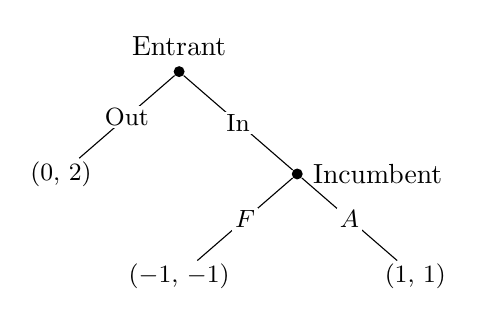
\begin{tikzpicture}[level distance=13mm, sibling distance=30mm]
\node[dec,label=above:{Entrant}] {}
  child { node[term] {$(0,\,2)$} edge from parent node[lab] {Out} }
  child { node[dec,label=right:{Incumbent}] {}
     child { node[term] {$(-1,\,-1)$} edge from parent node[lab] {$F$} }
     child { node[term] {$(1,\,1)$} edge from parent node[lab] {$A$} }
     edge from parent node[lab] {In} };
\end{tikzpicture}
\end{center}

\begin{itemize}
\item Strategies: $S_E=\{\text{Out},\text{In}\}$ and $S_I=\{F,A\}$. The Incumbent has a strategy
even when the Entrant stays out: it is what he \emph{would} do.
\item Normal form:
\begin{center}\small
\begin{tabular}{c|cc}
 & $F$ & $A$\\\hline
Out & $0,2$ & $0,2$\\
In & $-1,-1$ & $1,1$
\end{tabular}
\end{center}
\item Nash equilibria: $(\text{Out},F)$ and $(\text{In},A)$.
\item Backward induction: after In, $A$ (1) beats $F$ ($-1$); then In (1) beats Out (0).
\textbf{SPE: $(\text{In},A)$}, path In $\to A$, payoffs $(1,1)$.
\item $(\text{Out},F)$ is Nash only because of the \emph{off-path} instruction $F$, a threat that
is not credible. You can see this only if you wrote $F$ down.
\end{itemize}

\noindent\emph{Short-paper link.} Paper 1's leniency game has exactly this shape: the Applicant
chooses Propose or Not propose, then CADE chooses Accept or Reject. Its first SPE must be
written as the profile (Not propose, Accept), not just ``Not propose''.

\subsection{The follower moves at several nodes: replies are functions}

In the sequential Battle of the Sexes (Tadelis Fig.~7.7, p.~138), player 1 picks $O$ or $F$, and
player 2 observes it and picks $o$ or $f$. Player 2 has \emph{two} information sets, so
\[
S_2=\{oo,\ of,\ fo,\ ff\}\qquad(\text{p.~139}),
\]
where $of$ means ``$o$ after $O$, $f$ after $F$'' (``follow player 1'') and $fo$ means ``do the
opposite''. The two actions become four strategies because there are two information sets.

\begin{rulebox}[General count]
If the leader has $m_1$ actions and the follower observes them and has $m_2$ replies at each, the
follower has $m_2^{\,m_1}$ strategies, one reply \emph{for each} leader move. It is not
$m_1\times m_2$. Example: 3 leader moves and 2 replies give $2^3=8$ follower strategies, written
$(x,y,z)$ = (reply to $U$, reply to $M$, reply to $D$).
\end{rulebox}

\subsection{A player who moves twice (illustration)}

\begin{center}
\begin{tikzpicture}[level distance=13mm, sibling distance=32mm]
\node[dec,label=above:{P1}] {}
  child { node[term] {$(2,\,0)$} edge from parent node[lab] {Out} }
  child { node[dec,label=right:{P2}] {}
     child { node[term] {$(1,\,2)$} edge from parent node[lab] {$l$} }
     child { node[dec,label=right:{P1}] {}
        child { node[term] {$(3,\,1)$} edge from parent node[lab] {$a$} }
        child { node[term] {$(0,\,0)$} edge from parent node[lab] {$b$} }
        edge from parent node[lab] {$r$} }
     edge from parent node[lab] {In} };
\end{tikzpicture}
\end{center}

\begin{itemize}
\item P1 has \textbf{two} information sets (the root and the node after $r$). With the key ``(first
move, second move)'', $S_1=\{(\text{Out},a),(\text{Out},b),(\text{In},a),(\text{In},b)\}$, so
$2\times2=4$ strategies. $(\text{Out},a)$ and $(\text{Out},b)$ are \emph{different} strategies even
though Out ends the game (Tadelis p.~158 makes the same point with $NO$, $NF$).
\item P2 has one set: $S_2=\{l,r\}$.
\item Normal form (rows P1, columns P2):
\begin{center}\small
\begin{tabular}{c|cc}
 & $l$ & $r$\\\hline
$(\text{Out},a)$ & $2,0$ & $2,0$\\
$(\text{Out},b)$ & $2,0$ & $2,0$\\
$(\text{In},a)$ & $1,2$ & $3,1$\\
$(\text{In},b)$ & $1,2$ & $0,0$
\end{tabular}
\end{center}
\item Nash equilibria: $\big((\text{Out},a),\,l\big)$ and $\big((\text{Out},b),\,l\big)$. They have
the same path (Out) and the same payoffs $(2,0)$.
\item Backward induction: at P1's last node $a$ (3) beats $b$ (0); P2 then compares $l$ (2) with
$r\to a$ (1) and picks $l$; P1 compares Out (2) with In $\to l$ (1) and picks Out.
\textbf{SPE: $\big((\text{Out},a),\ l\big)$.}
\item Only the \emph{unreached} instruction separates the two equilibria: $b$ is not optimal
where it would be played, so $\big((\text{Out},b),l\big)$ is Nash but not subgame perfect. If you
had written P1's strategy as just ``Out'', you could not tell them apart.
\end{itemize}

%=====================================================================
\section{Imperfect information and multistage games}

\paragraph{One action per information set.} If player 2 does \emph{not} observe player 1's move,
for example in the simultaneous Battle of the Sexes drawn as a tree, player 2's two nodes form one
information set. Then $S_2=\{o,f\}$, only two strategies (Tadelis p.~139). The same action must be
played at every node of a set, because the player cannot tell the nodes apart.

\paragraph{Multistage games.} If both players move simultaneously in stage 1, see the outcome,
then move simultaneously in stage 2, a strategy is:
\[
\big(\text{stage-1 action};\ \text{stage-2 action after each stage-1 outcome}\big).
\]
In the two-stage prisoner's dilemma that is $1+4=5$ instructions, and in a two-stage game with a
$3\times3$ stage game it is $1+9=10$ (Gibbons p.~93). So each player in the two-stage PD has $2^5=32$
pure strategies.

%=====================================================================
\section{Mixed versus behavioral strategies}

\begin{itemize}
\item \textbf{Mixed} (Definition 7.5, p.~139): a probability distribution over \emph{whole plans}.
For player 2 in the sequential BoS: $(p_{oo},p_{of},p_{fo},p_{ff})$, summing to 1.
\item \textbf{Behavioral} (Definition 7.6, p.~140): an independent randomization \emph{at each
information set}, e.g. $\sigma_2(o\mid O)=\tfrac13$, $\sigma_2(o\mid F)=\tfrac12$.
\item With perfect recall they are equivalent (Kuhn; p.~142). Conversion:
$\Pr(o\mid O)=p_{oo}+p_{of}$ and $\Pr(o\mid F)=p_{oo}+p_{fo}$ (p.~141). In extensive-form answers,
write the behavioral form: ``at $h$, play $o$ with probability $q$''.
\end{itemize}

%=====================================================================
\section{Repeated games: strategies are functions of the history}

A strategy maps every possible history into a stage-game action (Tadelis Definition 10.4,
p.~196): $s_i:H\to S_i$. A strategy is an infinite list, so we write a \emph{rulebox} that covers
every history in one sentence. The rule must cover histories with deviations too: those are the
off-path information sets of the repeated game.

\begin{tmpl}[{Grim trigger, written completely (Tadelis p.~198; stage game $(M,m)=(4,4)$, $(M,f)=(-1,5)$, $(F,m)=(5,-1)$, $(F,f)=(1,1)$)}]
\textbf{Player 1:} in stage 1 play $M$. In any stage $t>1$, play $M$ if and only if every past
outcome was $(M,m)$; otherwise play $F$.\\
\textbf{Player 2:} the mirror rule with $m$ and $f$.\\[2pt]
Equilibrium statement: ``(grim trigger, grim trigger) is a subgame-perfect equilibrium iff
$\delta\ge \frac{T-R}{T-P}=\frac{5-4}{5-1}=\frac14$.''
\end{tmpl}

\noindent Other rules:
\begin{itemize}
\item \textbf{Tit-for-tat:} play $M$ in stage 1; in stage $t>1$ play whatever the opponent played in
stage $t-1$.
\item \textbf{Two-state machine} (an equivalent way to write grim trigger):
\begin{itemize}
\item State \emph{Cooperate}: play $(M,m)$, and move to \emph{Punish} after any other outcome.
\item State \emph{Punish}: play $(F,f)$ forever.
\end{itemize}
\end{itemize}

\begin{trap}[Classic error]
``Both play $M$ every period'' is a \emph{path}, not a strategy. It says nothing about what happens
after a deviation, so the incentive to cheat cannot be checked.
\end{trap}

%=====================================================================
\section{Bayesian games: one action for every type}

A pure strategy is a function from types to actions (Tadelis Definition 12.3, p.~249):
$s_i:\Theta_i\to A_i$. A type is an information set chosen by Nature, so the rule is the same as
before: plan for \emph{every type}, including the types not drawn. Player $j$ needs them to
compute expected payoffs. Count: $|A_i|^{|\Theta_i|}$.

\paragraph{Example (Tadelis pp.~243--244, p.~250).} An entrant chooses $O$ (stay out) or $E$
(enter). The incumbent is rational with probability $p$ or ``crazy'' (likes fighting) with
probability $1-p$, and chooses $A$ (accommodate) or $F$ (fight).
\begin{itemize}
\item The incumbent's strategy is written $xy$, with $x$ the rational type's action and $y$ the
crazy type's: $S_2=\{AA,AF,FA,FF\}$, so $2^2=4$.
\item The entrant has one type, so its strategy is a plain action: $\{O,E\}$.
\item At $p=\tfrac23$, against $E$ the incumbent's best strategy is $AF$ (payoff $\tfrac43$), and
against $AF$ entering pays the entrant $\tfrac13>0$. So $(E,\ AF)$ is a Bayesian Nash equilibrium,
written with \emph{both} types' actions.
\end{itemize}

\paragraph{Pooling and separating} (Gibbons p.~150). A strategy is \emph{separating} if different
types take different actions ($AF$, $FA$), and \emph{pooling} if all types take the same action
($AA$, $FF$).

\paragraph{Auctions (Lecture 8).} A type is a value $v_i$, so a strategy is a \emph{bid function}
$b_i(v_i)$ defined for every possible value, not a single number. Examples: in a second-price
auction, $b_i(v_i)=v_i$ for all $v_i$ (weakly dominant); in a first-price auction with two bidders
and values uniform on $[0,1]$, the symmetric equilibrium is $b(v)=v/2$ (Tadelis Ch.~13).

%=====================================================================
\section{Signaling games and PBE: strategies \emph{and} beliefs}

Following Gibbons §4.2.A (pp.~183--188), take a Sender with types $t_1,t_2$, messages $m\in\{L,R\}$,
and a Receiver who sees the message and picks $a\in\{u,d\}$.
\begin{itemize}
\item \textbf{Sender strategy}, one message per type: $(m(t_1),m(t_2))$. There are four:
$(L,L)$ and $(R,R)$ are pooling; $(L,R)$ and $(R,L)$ are separating.
\item \textbf{Receiver strategy}, one action per message, \emph{including a message nobody sends}:
$(a(L),a(R))$. There are four: $(u,u),(u,d),(d,u),(d,d)$.
\item \textbf{Beliefs}, for each message: $\mu(t_1\mid L)$ and $\mu(t_1\mid R)$. On the path they
come from Bayes' rule. After an unused message they are free, but the Receiver's action there
must be optimal given them.
\end{itemize}

\begin{tmpl}[How to write a PBE (format)]
``Sender plays $(L,L)$ (both types send $L$); Receiver plays $(u,d)$ ($u$ after $L$, $d$ after $R$);
beliefs $\mu(t_1\mid L)=p$ (Bayes, pooling) and $\mu(t_1\mid R)=q$ for any $q$ that makes $d$
optimal after $R$.''\\
All three parts are required: the Sender's strategy, the Receiver's strategy and the beliefs.
\end{tmpl}

%=====================================================================
\section{Common mistakes}

\begin{enumerate}
\item \textbf{Writing the path instead of the profile.} ``Out'' instead of $\big((\text{Out},a),l\big)$.
\item \textbf{Writing the payoffs as the equilibrium.} $(2,0)$ is the outcome's payoff, not the
equilibrium.
\item \textbf{Dropping off-path instructions.} They are exactly what subgame perfection tests.
\item \textbf{No key for the tuple.} $(F,A)$ is ambiguous unless you say which node each entry
belongs to.
\item \textbf{Same label at two nodes.} Use primes ($F$, $F'$) or ``after X''.
\item \textbf{Different actions inside one information set.} Not allowed: the player cannot tell
the nodes apart.
\item \textbf{Adding instead of multiplying.} The count is a product (or $m_2^{m_1}$ for replies).
\item \textbf{Repeated games: stating only cooperation.} The rule must say what happens after
\emph{any} deviation.
\item \textbf{Bayesian games: one action for the informed player.} Give one action per type, also
for the types not drawn.
\item \textbf{Signaling: forgetting the reply to the unused message, or the beliefs.}
\item \textbf{Mixing up mixed and behavioral.} Mixed randomizes over plans; behavioral randomizes
at each node.
\end{enumerate}

%=====================================================================
\section{Templates to copy}

\begin{tmpl}[Fill in the blanks]
\begin{tabular}{@{}p{3.6cm}p{11.2cm}@{}}
Extensive form & $s_i=(\text{action at }h_1,\ \text{action at }h_2,\dots)$ \quad key: $h_1=$ \underline{\hspace{1.5cm}}, $h_2=$ \underline{\hspace{1.5cm}}\\[2pt]
Profile & $(s_1;\ s_2)$; then ``path: \underline{\hspace{1.5cm}}, payoffs: \underline{\hspace{1.5cm}}''\\[2pt]
Repeated game & ``At $t=1$ play \underline{\hspace{1cm}}. At $t>1$: if the history is \underline{\hspace{2cm}}, play \underline{\hspace{1cm}}; otherwise play \underline{\hspace{1cm}}.''\\[2pt]
Bayesian & $s_i=(\text{action if }\theta^1,\ \text{action if }\theta^2,\dots)$\\[2pt]
Auction & $b_i(v)=$ \underline{\hspace{1.5cm}} for every $v$\\[2pt]
Signaling (PBE) & Sender $(m(t_1),m(t_2))$; Receiver $(a(m_1),a(m_2))$; beliefs $\mu(\cdot\mid m_1)$, $\mu(\cdot\mid m_2)$
\end{tabular}
\end{tmpl}

%=====================================================================
\section{Self-check (original practice on this guide's examples)}

\begin{enumerate}
\item In the ``player who moves twice'' game, list P1's pure strategies. How many are there?
\item Write that game's SPE as a full profile, then its path and payoffs.
\item Why is $\big((\text{Out},b),l\big)$ a Nash equilibrium but not an SPE?
\item The leader has 3 actions; the follower observes and has 3 replies at each node. How many
strategies does the follower have? And if the follower does \emph{not} observe?
\item How many instructions does a strategy have in a two-stage game whose stage game is $3\times3$?
\item Write tit-for-tat for player 2 in the labels $m,f$.
\item An informed player has 3 types and 2 actions. How many pure strategies does it have?
\item In the signaling game of Section 7, count the Sender's and the Receiver's strategies. What
else must a PBE state?
\item Write the SPE of Paper 1's leniency game (Applicant: Propose/Not propose; CADE: Accept/Reject;
CADE accepts after a proposal; the Applicant does not propose).
\end{enumerate}

\noindent\textbf{Answers.}
(1)~$(\text{Out},a),(\text{Out},b),(\text{In},a),(\text{In},b)$: four.
(2)~$\big((\text{Out},a),\,l\big)$; path Out; payoffs $(2,0)$.
(3)~Its path is a best response, but $b$ is not optimal at P1's second node ($0<3$).
(4)~$3^3=27$; without observing, 3.
(5)~$1+9=10$.
(6)~Play $m$ in stage 1; in stage $t>1$ play $m$ if player 1 played $M$ in $t-1$, and $f$ if they
played $F$.
(7)~$2^3=8$.
(8)~4 and 4; the beliefs after each message.
(9)~$(\text{Not propose},\ \text{Accept})$.

%=====================================================================
\section{Reading route}
\small
\begin{itemize}
\item Tadelis §7.2 (pp.~137--142): pure, mixed and behavioral strategies and counting; Ch.~8
(pp.~151--174): backward induction and SPE; §10.2--10.3 (pp.~193--200): histories, strategies,
grim trigger; §12.1--12.2 (pp.~241--257): type-contingent strategies; Ch.~13 (pp.~270--287): bid
functions; Ch.~15--16 (pp.~303--338): PBE and signaling.
\item Gibbons pp.~117--118 (why plans must be complete), p.~93 (multistage strategies), §4.2.A
(pp.~183--190, signaling strategies and beliefs).
\item Course notes: \texttt{Notas/L03/L03-02-strategies.md}, \texttt{L05-03}, \texttt{L05-04},
\texttt{L07-02}, \texttt{L08-04}.
\item Practice with full statements and worked solutions:
\texttt{Listas/lista-reais-lecture-03.pdf} and its solutions (trees, information sets and
strategies).
\end{itemize}

\end{document}
